\chapter{General principles}

\section{Kinematics}\marginnote{This somehow creates  playing field}

\subsection{Deformations}

Let \(\Omega\subset\R^n\) be a \dhighlight{domain} \marginnote{Open, connected set}.

\begin{definition}\label{def:1.1}
    A \(C^k\) (\(k\geq 1\)) deformation of a domain \(\Omega\subset\R^n\) is a map \(\varphi:\Omega\to\R^n\) with:
    \begin{enumerate}
        \item \(\varphi\in C^k(\Omega,\R^n)\) 
        \item \(\varphi\) has a continuous extension to \(\overline{\Omega}\) and the extension is invertible
        \item \(\varphi\) is \dhighlight{orientation preserving}: \(\det D\varphi>0\) in \(\Omega\).
    \end{enumerate}
    \(\Omega\) is often called the \dhighlight{reference configuration} of the body and \(\varphi(\Omega)\) is often called 
    the \dhighlight{deformed configuration} (position in physical space).
\end{definition}

\subsubsection*{Some linear algebra}%TODO

Simplest example: \(\varphi(x)=Ax+b\) with \(b\in \R^n, A:\R^n\to\R^n\) linear with \(\det A>0\).
We often identify linear maps with the corresponding matrix with respect to the standard basis of \(\R^n\).
\[Ae_j=\sum_{i=1}^nA_{ij}e_i\]
We also usually use the standard scalar product on \(\R^n\)
\[x\cdot y=\sum_{i=1}^n x_iy_i\]

Transpose is defined by 
\[A^\intercal x\cdot y=x\cdot A y\]
for all \(x,y\in\R^n\).

\(A\) is symmetric if \(A^\intercal =A\). A symmetric matrix \(A\) is positive semi-definite if 
\[Ax\cdot x\geq 0\]
and positive definite if 
\[Ax\cdot x> 0.\]

\begin{definition}\label{def:1.2}
    \[O(n)=\{A:A^\intercal A=\Id\}\]
    \[\SO(n)=\{A:A^\intercal A=\Id, \det A=1\}\]
\end{definition}

Some basic facts: 
\begin{itemize}
    \item \(A\) isometry: \(|Ax|^2=|x|^2\forall x\in \R^n\) which holds \(\iff A\in O(n)\)
    \item \(A\in O(n)\implies \det A = \pm 1\)
\end{itemize}

Norms on matrices:
\begin{itemize}
    \item \dhighlight{Euclidean norm (Hilbert Schmidt norm)}: \(|A|^2=\text{tr}(A^\intercal A)=\sum_{i,j=1}^n A_{ij}^2, A\cdot B=\text{tr}A^\intercal B\)
    \item \dhighlight{Operator norm} \(\Vert A \Vert = \supp_{x\neq 0} \frac{|Ax|}{|x|}=\sup_{|x|=1}|Ax|\implies \Vert AB\Vert \leq \Vert A\Vert\Vert B\Vert \)
\end{itemize}

\begin{lemma}[Polar decomposition]\label{lem:1.3}
    Let \(A:\R^n\to\R^n\) linear, \(\det A>0\).
    \begin{enumerate}
        \item There exists a unique pair \((R,U)\) with \(R\in \SO(n), U\) symmetric s.t. \[A=RU\]
        \item there exists a unique pair \((R',V)\) with \(R'\in \SO(n), U\) symmetric s.t. \[A=VR'\]
    \end{enumerate}
    If \(\det A=0\) this is still possible, but we lose uniqueness.
\end{lemma}

\begin{theorem}\label{thm:1.4}
    Let \(W\) be symmetric and positive semi-definite. 
    Then there exists a unique symmetric and positive semi-definite matrix \(U\), such that \[W=U^2.\] 
\end{theorem}
\dhighlight{Notation:} \(U=\sqrt{W},U=W^{\frac{1}{2}}\).

\begin{proof}
    Just existence(not uniqueness).

    Let \(D=\text{diag}(d_i),d_i\geq 0\), then \(D^{\frac{1}{2}}=\text{diag}(\sqrt{d_i})\).
    For \(W\) symmetric positive definite, we get \[W=Q^\intercal D Q, Q\in \SO(n)\]
    Then \(U=Q^\intercal D^{\frac{1}{2}}Q\) is the square root: \[U^2=Q^\intercal D \underbrace{QQ^\intercal}_{=\Id}\] 
\end{proof}

\begin{proof}[Proof of \ref{lem:1.3}]
    For (ii) apply (i) to \(A^\intercal\).

    For (i): Assume we already knew that there are \((R,u)\) s.t. \[A=RU.\]
    Then \begin{align*}
        A^\intercal & = U^\intercal R^\intercal = UR^\intercal \\
        A^\intercal &A = U \underbrace{R^\intercal R}_{=\Id} U = U^2\\
        (A^\intercal A)^\intercal&=A^\intercal A \\
        (A^\intercal A x\cdot x &= (Ax\cdot A x)\geq 0)\\
        &\implies U=(A^\intercal A)^\frac{1}{2}
    \end{align*}

    If such a decomposition exists, \(U\) is unique by the formula.

    For existence define \(U=(A^\intercal A)^\frac{1}{2}\) and \(R\coloneqq AU^{-1}\). We have to 
    check that \(R\in \SO(n)\):
    \begin{align*}
        R^\intercal R &=(U^{-1})^\intercal A^\intercal A U^{-1}=\Id\\
        \det R &=\det A \det (U^{-1})>0\implies R\in \SO(n).
    \end{align*}
\end{proof}

\begin{lemma}\label{lem:1.5}
    \(A\in \R^{n\times n}\). Then there exists \(R,Q\in \SO(n)\) and \(\lambda_1\in \R,\lambda_2,\dots,\lambda_n\geq 0\) s.t. \(|\lambda_1|\leq \lambda_2\leq \dots \leq \lambda_n\):
    \[A=R\begin{bmatrix}
        \lambda_1 &&\\
        &\ddots & \\
        &&\lambda_n
    \end{bmatrix} Q.\]
    The \(\lambda_1,\dots,\lambda_n\) are uniquely determined by \(A\). The \(\lambda_i\) are called 
    the singular values of \(A\).
\end{lemma}

\begin{proof}
    If \(\det A>0\stackrel{\implies}{\text{Polar decomp.}} A=RU=\underbrace{R'Q^\intercal}_{R\in \SO(n)} D Q\).

    If \(\det A<0\) consider \(P=\begin{bmatrix}
        -1 & &&\\
        & 1 &&\\
        &&\ddots&\\
        &&&1
    \end{bmatrix}\implies \det(AP)>0\).

    The \(\vert A^\intercal A\vert\) are the eigenvalues of \((A^\intercal A)^\frac{1}{2}\).

\end{proof}

We know \(|A|=(\sum_{i=1}^n \lambda_i^2)^\frac{1}{2},\Vert A \Vert = \lambda_n\) and 
\[\det A=\prod_{i=1}^n \lambda_i\]

\subsubsection*{Rigid motion}


\begin{definition}\label{def:1.6}
    A deformation \(\varphi:\Omega\to \R^n\) is called a \dhighlight{rigid deformation} if \(D\varphi(x)\in \text{SO}(n)\forall x\in \Omega\).
\end{definition}

\begin{theorem}[Liouville]\label{thm:1.7}
    Suppose \(\varphi:\Omega\to\R^n\) is \(C^1\), \(\Omega\) is a domain and \(\det D\varphi\). Then the following three statements are equivalent:
    \begin{enumerate}
        \item \(D\varphi(x)\in\text{SO}(n)\forall x\in \Omega\) (Rigid motion)
        \item \(\varphi\) is an \dhighlight{affine} rigid motion: \[\varphi(x)=Ax+b, A\in \text{SO}(n),b\in \R^n\]
        \item \(|\varphi(x)-\varphi(y)|=|x.y|\forall x,y\in \R^n\)
    \end{enumerate} 
\end{theorem}

\begin{proof}
    Ideas (rest is homework):

    \begin{itemize}
        \item (ii) \(\implies\) (iii) is clear (since we assume the determinant to be $>0$)
        \item (iii) \(\implies\) (ii): nice ex. (true in hilbert spaces). \(\varphi((1-\lambda)x+\lambda y)=(1-\lambda)\varphi(x)+\lambda\varphi(y)\) By using that spheres are mapped to spheres (and two of those intersect in a single point)
        \item (ii) \(\implies\) (i): trivial
        \item (i) \(\implies\) (ii): goes via local version of (iii). Claim: for all \(x_0\in\Omega\exists r>0, B_r(x_0)\subset \Omega\) and \(|\varphi(x)-\varphi(y)|\leq |x-y|\forall x,y\in B_(0)\)
        \item \(\geq \)Use inverse function theorem 
    \end{itemize}
\end{proof}

This can be generalized to Sobolev spaces.

\markeol{01}

\beginlecture{02}{11.04.2025}

\dhighlight{Organization}

The tutorial will be \dhighlight{mondays 08-10} First tutorial on  April 28th.

Homework: Sheet 01 (Half sheet) on his homepage under teaching. Hand in on April 18th

Sheet 02: out on Wednesday April 16th due on April 23rd

\begin{figure}[H]\label{fig:1.01}
    \centering
    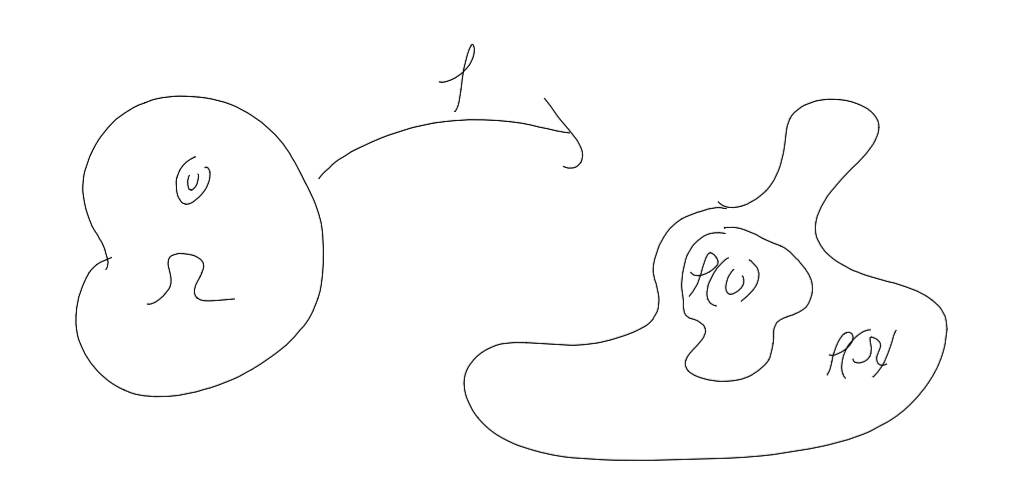
\includegraphics[width=.7\textwidth]{fig_1_01.png}
    \caption{Sketch 1.01}
\end{figure}

Change of volume from \(U\to \varphi(U)\) and the change of surface area from \(\partial U \to \partial \varphi(U)\)

\subsubsection*{Change of volume /area for linear maps}

\(A:\R^n\to\R^n\) linear, \(E\subset\R^n\)
\[\mathcal{L}^n(AE)=|\det A|\mathcal{L}^n(E)\]

Now \(B:\R^{n-1}\to\R^n\) linear, \(E\subset\R^{n-1}\)
\[\mathcal{H}^{n-1}(BE)=\sqrt{\det B^\intercal B} \underbrace{\mathcal{H}^{n-1}(E)}_{\mathcal{L}^{n-1}(E)}\]

\begin{proof}[Proof sketch]
    \(Q:\R^{n-1}\to\R^n\) linear and isometric. Then 
    \[\mathcal{H}^{n-1}(QE)=\mathcal{H}^{n-1}(E).\]
    Polar decomposition: (first assume \(B\) has max rank \(n-1\)). Then \(B^\intercal B:\R^{n-1}\to\R^{n-1}\) is invertible and 
    \[B=Q(B^\intercal B)^{\frac{1}{2}}\]
    with \(Q=B\left((B^\intercal B)^{\frac{1}{2}}\right)^{-1}\). We can check that \(Q^\intercal Q=\Id\), i.e. 
    \(Q\) is an isometry.
    \[\mathcal{H}^{n-1}(BE)=\mathcal{H}^{n-1}((B^\intercal B)^{\frac{1}{2}}E)=\sqrt{\det B^\intercal B} \mathcal{H}^{n-1}(E)\qedhere\]
\end{proof}

\begin{definition}\label{def:1.8}
    Let \(A\in \R^{n\times n}\) the \dhighlight{cofactor matrix} \(\text{cof}(A)\) is defined by 
    \[\text{cof}(A)_{i,j}=(-1)^{i+j}\det B^{ij},\]
    where \(B^{ij}\) is the matrix obtained by deleting the ith row and jth column from \(A\).
\end{definition}

\begin{align*}
    A&=\begin{bmatrix}
        A_{11} & A_{12}\\
        A_{21} & A_{22}
    \end{bmatrix}\\
    \text{cof}(A) &= \begin{bmatrix}
        A_{22} & -A_{21}\\
        -A_{12} & A_{11}
    \end{bmatrix}
\end{align*}

\dhighlight{Ana 2:} \(f(A)=\det A\), then \[\frac{\partial f}{\partial A_{ij}}=(\text{cof}(A))_{i,j}.\]

\begin{lemma}[Cramer's rule]\label{lem:1.9}
    \begin{enumerate}
        \item \(A^\intercal \text{cof} A = \det{A}\Id\) If \(A^{-1}\) exists: \(A^{-1}=\frac{(\text{cov} A)^\intercal}{\det A}\)
        \item \(\det \text{cof} A=(\det A)^{n-1}\)
        \item \(\text{cof} A = (\det A)A^{-\intercal}\) if \(A\) is invertible
        \item \(\text{cof} A = A\) if \(A\in \SO(n)\)
        \item \(\text{cof}(AB)=(\text{cof}A)(\text{cof}(B))\)
    \end{enumerate}
\end{lemma}

\begin{proof}
    Linear algebra
\end{proof}

\begin{lemma}\label{lem:1.10}
    Let \(A\in \R^{n\times n}, H\subset \R^n\) be a \(n-1\) dimensional subspace with normal \(nu\).
    Then 
    \begin{enumerate}
        \item \((\text{cof} A)\nu\neq 0\) then \(AH\) is also an \(n-1\) dimensional subspace. 
            If, in addition \(\det A\geq 0\) then \(A\) maps the half space \(\{x:x\cdot\nu\leq 0\}\) to the subspace 
            \(y:y\cdot (\text{cof}A)\nu\leq 0\). If \((\text{cof}A)\nu=0\) then \(AH\) has dimension \(\leq n-1\).
        \item Let \(\bar{A}=A\restrict{H},\bar{A}:H\to\R^n\). Define \(\bar{A}^\intercal: \R^n\to H\) by 
            \(\bar{A}^\intercal x \cdot y \coloneqq x \cdot \bar{A} y\) for all \(x\in \R^n,y\in H\). Then 
            \[\det\left(\bar{A}^\intercal\bar{A}\right)=\vert (\text{cof}A)\nu\vert^2\]
        \item \(\mathcal{H}^{n-1}(AE)=(\det \bar{A}^\intercal \bar{A})^{\frac{1}{2}}\mathcal{H}^{n-1}(E)=|\text{cof A} \nu|\mathcal{L}^{n-1}(E)\)    
    \end{enumerate}
\end{lemma}

\begin{figure}[H]\label{fig:1.02}
    \centering
    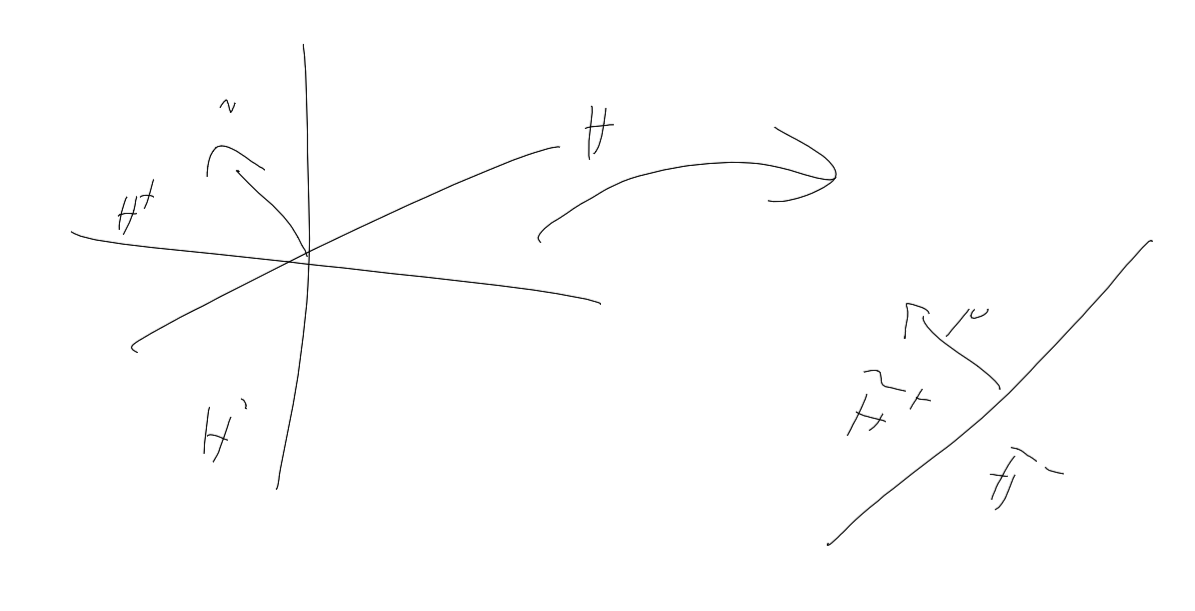
\includegraphics[width=.7\textwidth]{fig_1_02.png}
    \caption{Sketch 1.02}
\end{figure}

\begin{proof}
Exercise. Hints:
\begin{enumerate}
    \item It is often a good idea to look at a special case: \(H=\R^{n-1}\times \{0\},\nu=e_n\)
        \((\text{cof} A) e_n=\begin{bmatrix}
            (\text{cof} A)_{1n}\\ \vdots\\ (\text{cof} A)_{nn}
        \end{bmatrix}\) This gives the first part.
    \item General case: Consider \(Q\in \SO(n)\) \[Qe_n=\nu, \ Q(\R^{n-1}\times \{0\})=H.\] Then use \[\text{cof Q}=Q,\ \text{cof}(QA)=\text{cof} Q\text{cof }A.\] 
\end{enumerate}    
\end{proof}

\begin{theorem}\label{thm:1.11}
    Let \(\Omega\in\R^n\) be a domain, \(\varphi:\Omega\to\R^n\) a \(C^1\) deformation. Then 
    \begin{enumerate}
        \item For all measurable \(U\subset\Omega\) and for all \(g\in L^1(\varphi(U))\). 
        \[\int_{\varphi}(U)g(x)dx\int_U g(\varphi(X))=\det D\varphi(X)dX\]
        \item For all bounded sets \(U\subset \Omega\) with a \(C^1\) boundary and \(\bar{U}\subset \Omega\) and all \(g\in L^1(\varphi(\partial U))\)
            \[\int_{\partial \varphi(U)}g(x)d\mathcal{H}^{n-1}(x)=\int_{\partial U} g(\varphi(X))|\cof D\varphi(X)\nu(X)|d\mathcal{H}^{n-1}(X)\]
            \[\int_{\partial \varphi(U)}g(x)\underbrace{\mu(x)d\cH^{n-1}(x)}_{\text{oriented area}}=\int_{\partial U}g(\varphi(X))\cof D\varphi(X)\nu(X)d\mathcal{H}^{n-1}(x)\]
    \end{enumerate}
\end{theorem}

\begin{figure}[H]\label{fig:1.03}
    \centering
    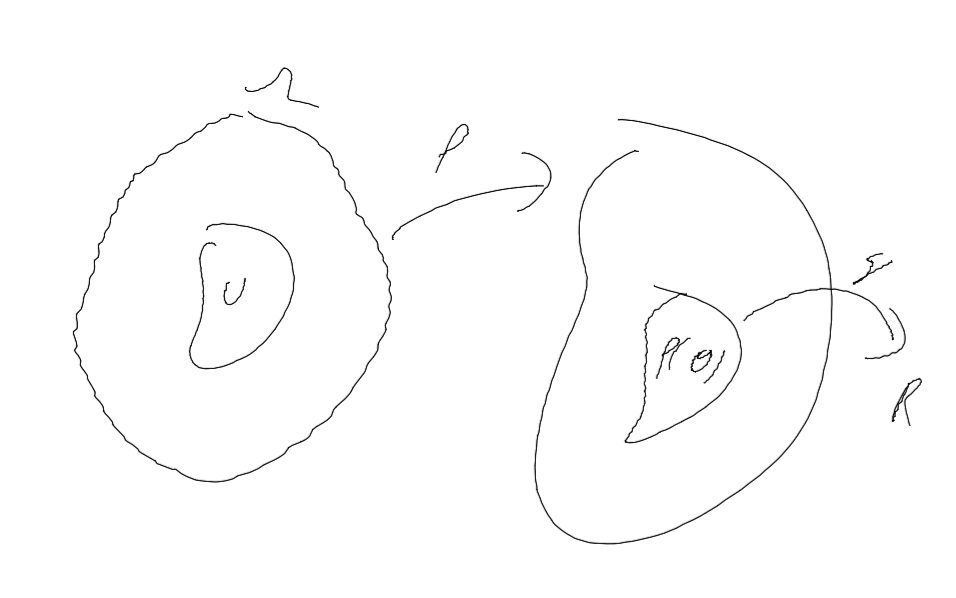
\includegraphics[width=.7\textwidth]{fig_1_03.png}
    \caption{Sketch 1.03}
\end{figure}

\begin{proof}
    (i) Analysis 3 (ii) using charts and partition of unity.
\end{proof}

\subsection{Motions, material time derivative}

\dhighlight{Motivation:}

\begin{figure}[H]\label{fig:1.04}
    \centering
    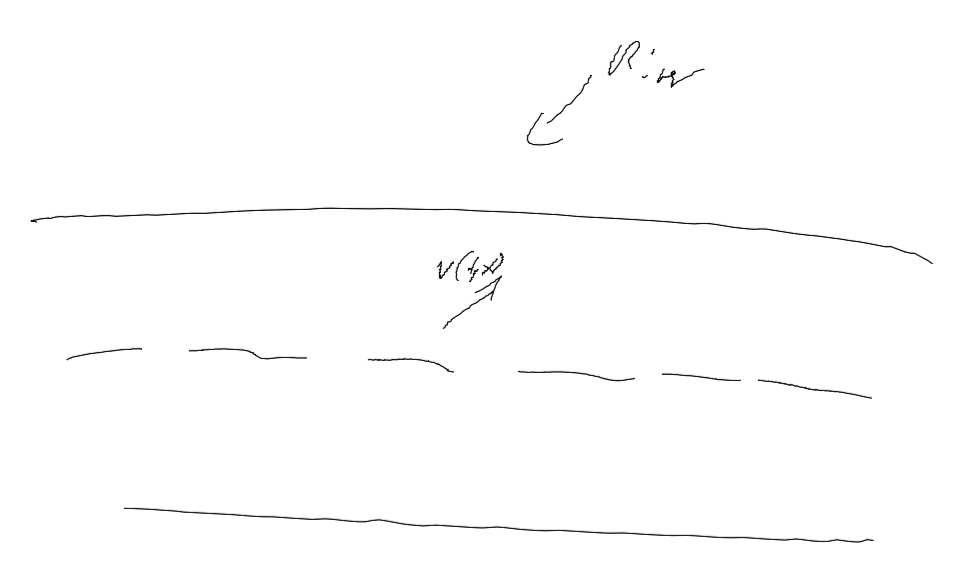
\includegraphics[width=.7\textwidth]{fig_1_04.png}
    \caption{Sketch 1.04}
\end{figure}
where \(v(t,x)\) is the \dhighlight{velocity} at spacial point \(x\) and time \(t\).
\[\frac{\partial v}{\partial t}(t,x)\]
Change of velocity at spacial point \(x\) and time \(t\). But this is \highlight{not} what we usually mean by acceleration!
Particles follow a certain path. To get what happens we need to follow the particle!

\begin{definition}\label{def:1.12}
    Let \(\Omega\subset\R^n\) a domain, A \dhighlight{motion} is a \(C^3\) map \(\varphi:\underbrace{\R}_{\text{time}}\times \Omega\to\R^n\) s.t. 
    for every \(t\in\R\) the map \(\varphi_t:\Omega\to\R^n\) defined by \[\varphi_t(x)\coloneqq \varphi(t,x)\]
    is a \(C^2\) deformation.

    \begin{enumerate}
        \item \(\Omega_t=\varphi_t(\Omega)\). The set which the body occupies in physical space at time \(t\)
        \item \(\tau=\{(t,x),t\in \R,x\in\Omega_t\}\) is the \dhighlight{trajectory} or \dhighlight{trail} in space time %TODO: This should be a script tau?
        \item \(\Phi_t=\varphi_t^{-1}:\Omega_t\to\Omega\). This is called the \dhighlight{back to labels map at time \(t\)}
        \item \(\Phi:\tau\to\R^\times\Omega\). \(t,x\mapsto (t,\Phi_t(x))=(t,\varphi_t^{-1(x)})\)
    \end{enumerate}

\end{definition}

\begin{definition}\label{def:1.13}
    \begin{enumerate}
        \item A map \(G:\R \times \underbrace{\Omega}_{\text{reference configuration}}\to\R^n\) is a \dhighlight{material field}. Notation:
        \(\dot{G}\) denotes the partial derivative w.r.t. the first argument \(t\) and \(DG\) denotes the partial derivative w.r.t. the second argument \(x\)
        \item A map \(g:\tau\to\R^n\) is called a \dhighlight{spacial field}. \(g'\) denotes the partial derivate w.r.t. the first argument and \(Dg\) denotes he partial derivative w.r.t the second argument.
    \end{enumerate}
    Sometimes we write \(D_XG\) instead of \(DG\) and \(D_xg\) instead of \(Dg\).
\end{definition}

\begin{example}
    Motion \(q\) is a material field and \(\Phi\) is a spacial field.
\end{example}

\begin{definition}\label{def:1.14}
    \begin{enumerate}
        \item Let \(g:\mathcal{T}\to\R^n\) be a spacial field, define \(g_m(t,X)=g(t,\varphi_t(X))\). Then \(g_m:\R\times \Omega\to\R^d\) is a material field, called the \dhighlight{material description} of \(g\)
        \item Let \(G:R\times \Omega\to\R^n\) be a material field, define \(G_s(t,x)=G(t,\Phi_t(x))\) then \(G_s\) is the \dhighlight{spacial description} of \(G\)
    \end{enumerate}
\end{definition}

Motion \(\varphi\) is a material field. 
\begin{align*}
    v(t,x)&\coloneqq\frac{\partial}{\partial t}\varphi(t,X)\\
    a(t,X)&\coloneqq \frac{\partial}{\partial t} v(t,X)=\frac{\partial^2}{\partial t^2}\varphi(t,X)
\end{align*}
are the velocity and the acceleration.

\begin{definition}[Material time derivative, time derivate at a fixed material point]\label{def:1.15}
    Let \(G:\mathcal{T}:\to\R^m\) be a spacial field. The material time derivative, denoted b 
    \(\dot{g}\) is defined by 
    \begin{align*}
        \dot{g}\coloneqq \left(\frac{\partial }{\partial t} g_m\right)_s
    \end{align*}
\end{definition}

Define \(g_m(t,X)=g(t,\varphi_t(X))=g(t,\varphi(t,X))\).
\begin{align*}
    \dot{g}(t_0,x_0)=? & X_0=\Phi_t(x_0), x_0=\varphi_t(X_0)\\
    \frac{\partial}{\partial t} g_m(t_0,X_0) & = \frac{\partial g}{\partial t}(t_0,\varphi_{t_0}(X_0))+\sum_{i=1}^n\frac{\partial g}{\partial x_i}(t_0,\varphi_t(X_0))\frac{\partial \varphi_i}{\partial t}(t_0,X_0) \\
    \dot{g}(t_0,x_0)&=\left(\frac{\partial}{\partial t}g_m\right)(t_0,\Phi_t(x_0))(v_s)_{i}(t_0,x_0)\\
    \dot{g}(t_0,x_0)&= \frac{\partial g}{\partial t}(t_0,x_0)+\sum_{i}\frac{\partial g}{\partial x_i}(t_0,x_0)v_s(t_0,x_0)
\end{align*}

\begin{theorem}\label{thm:1.16}
    Let \(g\) be a \(C^1\) spatial field.
    \[\dot{g}=\frac{\partial g}{\partial t}+\underbrace{\sum (v_s)_i\frac{\partial g}{\partial x_i}}_{D_g v_s = v_s\cdot \nabla g}\]
\end{theorem}

Special case if we view the velocity as a spacial field:
\[\dot{v}=\frac{\partial v}{\partial t}+v\cdot \nabla v\]
is the acceleration and \(v\cdot \nabla v\) is the only non-linearity in Navier-Stokes and Euler.

\begin{definition}\label{def:1.17}
    A motion is \dhighlight{isochoric (volume preserving)} if for all open sets \(U\subset \Omega\) the map 
    \(t\mapsto \mathcal{L}^n(U_t)\) is constant, where \(U_t=\varphi_t(U)\). 
\end{definition}


Spoiler: we need \(t\mapsto \det D\varphi_t(x)\) is constant.

\markeol{02}